\chapter{Architetture proposte}
\label{chap_6}
Lo stato dell'arte per la classificazione di varie patologie è l'utilizzo di algoritmi di deep learning; in questo capitolo tratteremo le tre architetture implementate nel presente lavoro di tesi: un \textbf{Multi-Layer Perceptron} (MLP), una \textbf{Convolutional Neural Network} (CNN) monodimensionale e una \textbf{Graph Convolutional Network} (GCN) con backbone convoluzionale. Le tre architetture vengono presentate in ordine di complessità crescente, sia dal punto di vista strutturale sia da quello delle formulazioni matematiche necessarie alla loro comprensione. Per ognuna, gli iperparametri specifici (numero di layer, numero di neuroni/filtri, dimensione dei kernel, ecc.) sono stati determinati tramite ottimizzazione bayesiana con \textbf{Optuna}, ripetuta separatamente per ciascuna configurazione del problema, in funzione del tipo di inversione degli elettrodi da rilevare e del numero di classi del task di classificazione considerato.

\section{Multi-Layer Perceptron}
\label{sec:mlp}

Il \textbf{Multi-Layer Perceptron} (MLP) rappresenta l'architettura più semplice tra quelle proposte ed è stato utilizzato come modello di baseline. Si tratta di una rete neurale \textit{feed-forward} completamente connessa (\textit{fully connected}), in cui ogni neurone di un layer riceve in ingresso l'output di tutti i neuroni del layer precedente. La rete è organizzata in un layer di ingresso, uno o più layer nascosti e un layer di uscita, la cui dimensione dipende dal numero di classi del problema di classificazione affrontato. Il numero di layer nascosti e il numero di neuroni per layer sono stati determinati tramite ottimizzazione con Optuna, in funzione della specifica configurazione del task.

\subsection{Funzioni di Attivazione}

Le \textbf{funzioni di attivazione} introducono non-linearità nella rete, permettendo al modello di apprendere relazioni complesse tra i dati in input. Senza di esse, indipendentemente dal numero di layer, la rete si comporterebbe come un semplice modello lineare.

Le funzioni di attivazione più comuni sono:

\begin{itemize}
	\item \textbf{ReLU (Rectified Linear Unit)}: definita come $f(x) = \max(0, x)$, azzera tutti i valori negativi e lascia invariati quelli positivi. È la funzione più utilizzata grazie alla sua semplicità computazionale e alla sua efficacia nel ridurre il problema del \textit{vanishing gradient}.
	\item \textbf{Sigmoid}: definita come $f(x) = \frac{1}{1 + e^{-x}}$, mappa i valori in un intervallo $(0, 1)$. Viene tipicamente usata nell'ultimo layer per problemi di classificazione binaria.
	\item \textbf{Softmax}: estensione della sigmoid per problemi multi-classe, produce una distribuzione di probabilità sull'insieme delle classi: $f(x_i) = \frac{e^{x_i}}{\sum_j e^{x_j}}$.
\end{itemize}

\subsection{Funzione di Loss}

La \textbf{loss function} (funzione di costo) quantifica l'errore tra le previsioni del modello $\hat{y}$ e i valori reali $y$ nel training set. L'obiettivo dell'apprendimento è minimizzare questa funzione.

Le loss function più utilizzate sono:

\begin{itemize}
	\item \textbf{Cross-Entropy Loss} (per classificazione multi-classe): misura la distanza tra la distribuzione predetta e quella reale.
	\[
	\mathcal{L} = -\sum_{c=1}^{C} y_c \log(\hat{y}_c)
	\]
	dove $C$ è il numero di classi, $y_c \in \{0,1\}$ è il label reale e $\hat{y}_c$ è la probabilità predetta per la classe $c$.
	
	\item \textbf{Mean Squared Error} (per regressione):
	\[
	\mathcal{L} = \frac{1}{N} \sum_{i=1}^{N} (y_i - \hat{y}_i)^2
	\]
\end{itemize}

\subsection{Fondamenta matematiche}
In questa sezione richiameremo alcuni strumenti di calcolo differenziale, necessari per la comprensione dell'aggiornamento dei pesi di una rete tramite l'\textbf{algoritmo di backpropagation}:

\subsubsection{Chain Rule}
La chain rule è la formula fondamentale per il calcolo della derivata di una funzione composta. Siano $g:\mathbb{R}\to\mathbb{R}$ e $f:\mathbb{R}\to\mathbb{R}$ derivabili, allora $g\circ f:\mathbb{R}\to\mathbb{R}$ è anch'essa derivabile, e se poniamo $h(x)=g(f(x))$, abbiamo che:
\[
\frac{dh}{dx}=g'(f(x))\cdot f'(x)
\]
Espandendo il ragionamento, definiamo $q:\mathbb{R}\to\mathbb{R}$; allora $q\circ g\circ f:\mathbb{R}\to\mathbb{R}$ è derivabile, e ridefinendo $h(x)=q(g(f(x)))$ otteniamo:
\[
\frac{dh}{dx}=q'(g(f(x)))\cdot g'(f(x))\cdot f'(x)
\]

\subsubsection{Chain rule per funzioni di funzioni}

Consideriamo un vettore $x(t)=\big(x_1(t),x_2(t),\dots, x_n(t)\big)^T\in\mathbb{R}^n$, le cui componenti sono $n$ funzioni derivabili. Sia inoltre $f:\mathbb{R}^n \to\mathbb{R}$ una funzione differenziabile in $x(t)$.

Sotto queste ipotesi, la funzione composta $F(t) = f(x(t))$ risulta differenziabile in $t$, e la sua derivata si esprime attraverso la chain rule come:
\[
F'(t)=\sum_{i=1}^{n}\frac{\partial f(x(t))}{\partial x_i} \cdot x_i'(t)=\langle\nabla f(x(t)),x'(t)\rangle
\]
dove l'espressione finale denota il prodotto scalare tra il gradiente della funzione $f$ e il vettore derivato $x'(t)$.

A titolo di esempio, data una funzione che dipende da due componenti generiche, ovvero $f\big(h(t), g(t)\big)$, la derivata totale di $f$ rispetto al parametro $t$ si calcola come:
\[
\frac{df}{dt} = \frac{\partial f}{\partial h} \frac{dh}{dt} + \frac{\partial f}{\partial g} \frac{dg}{dt}
\]

\subsubsection{Gradiente}
Sia $A\subseteq\mathbb{R}^2$ aperto e $f:A\to\mathbb{R}$, se tutte le derivate parziali esistono e sono continue allora $f$ è differenziabile. Se $f$ è differenziabile allora le sue derivate parziali, (due in questo caso) in un punto $P$ arbitrario, formano un vettore chiamato gradiente:
\[
\nabla f(x_0,y_0)=\left[\frac{\partial f}{\partial x}(x_0,y_0)\,, \quad\frac{\partial f}{\partial y}(x_0,y_0)\right]
\]

\subsubsection{Derivata direzionale}
Sia $A\subseteq\mathbb{R}^2$ aperto e $f:A\to\mathbb{R}$ continua, definiamo la derivata direzionale $D_v$ come la variazione della funzione $f$ lungo la direzione di un \textbf{versore} $v$ a partire da un punto $P$ arbitrario; viene formalmente indicata come:
\[
D_vf(x_0,\,y_0)=\lim_{t\to 0}\frac{f(x_0+t\,v_x,\,y_0+t\,v_y)-f(x_0,\,y_0)}{t}
\]
Se $f$ è anche \textbf{differenziabile}, allora possiamo ricorrere al \textbf{Teorema del Gradiente} per calcolare la derivata direzionale:
\[
D_vf(x_0,\,y_0)=\nabla f(x_0,\,y_0)\cdot v
\]
Espandendo otteniamo:
\[
\left[\frac{\partial f}{\partial x}(x_0,y_0)\,, \quad\frac{\partial f}{\partial y}(x_0,y_0)\right]\cdot \def\arraystretch{1.0} \begin{pmatrix}
	v_x \\ v_y
\end{pmatrix}
\]
Ora vogliamo calcolare qual'è la direzione $v$ in cui $f$ ha crescita massima:
\[
D_vf(x_0,\,y_0)=||\nabla f(x_0,\,y_0)||\cdot||v||\cdot\cos(\alpha)
\]
dove $\alpha$ indica l'angolo tra il versore e il gradiente. Osservando che $||v||=1$ e $-1\le\cos(\alpha)\le 1$ possiamo dire che $D_vf(x_0,\,y_0)$ assume valore \textbf{massimo} quando $\cos(\alpha)=1\to\alpha=0$, cioè se $v$ ha stessa direzione e verso del gradiente; viceversa assume valore \textbf{minimo} quando $\cos(\alpha)=-1\to\alpha=\pi$, cioè quando $v$ ha stessa direzione ma verso opposto al gradiente.

\subsection{Algoritmo di Backpropagation}
Uno dei primi algoritmi proposti per il calcolo dei pesi in una rete neurale è il metodo iterativo noto come metodo di backpropagation. La riscoperta di questo metodo verso la metà degli anni '80 da parte di Rumelhart, Hinton e Williams ha reso possibile definire algoritmi di addestramento per reti multistrato, ed è stato quindi alla base del successivo sviluppo degli studi sulle reti neurali. L'algoritmo è legato essenzialmente alla tecnica utilizzata per il calcolo delle derivate della funzione di errore, basata sulle regole di derivazione delle funzioni composte.

\subsubsection{Percorso generale di esecuzione}

Prima di tutto, è necessario definire come \textbf{epoca} il compimento di una fase di training, cioè quando tutto il dataset di training è passato attraverso la rete. Il dataset di training viene suddiviso in piccoli \emph{batch} (dimensione 16, 32, 64 ecc.), per ognuno si procede con il calcolo della funzione di loss $L(y, \hat{y})$, per poi proseguire con il calcolo della funzione di costo:
\[
C(w)=\frac{1}{n_T}\sum_{j=1}^{n_T}L(y^{(j)},\hat{y}^{(j)}(w))
\]
dove $n_T$ rappresenta la dimensione del batch di training, e $y^{(j)},\hat{y}^{(j)}$ sono rispettivamente le etichette e le predizioni della rete al $j$-esimo esempio di training.
Infine dobbiamo aggiornare i pesi muovendoci in direzione dell'antigradiente per cercare di minimizzare la funzione di costo:
\[
w^{(k)}=w^{(k-1)}-\eta\nabla C(w)
\]
dove $\eta$ rappresenta il \textbf{learning rate} (tasso di apprendimento) che definisce di quanto dobbiamo muoverci verso la direzione dell'antigradiente; questo parametro è fondamentale per l'apprendimento delle reti, in quanto, con valori troppo piccoli, la convergenza della rete richiederebbe tempi troppo lunghi, quindi più energia consumata e più epoche, mentre valori troppo grandi potrebbero evitare che la rete converga, in quanto i punti di minimo che cerchiamo di ottenere potrebbero essere "saltati" direttamente.

\begin{figure}[h!]
	\centering
	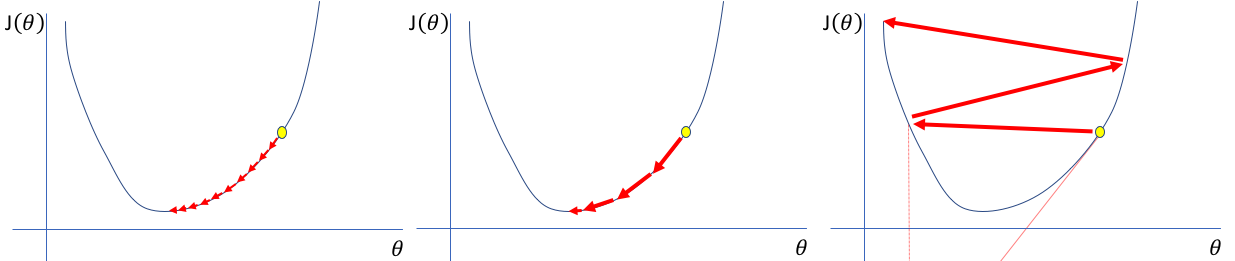
\includegraphics[width=0.9\linewidth]{images/lr_high_and_low.png}
	\caption{Differenza nella scelta del learning rate}
	\label{fig:lr_diff}
\end{figure}

\subsection{Calcolo del Gradiente in un MLP}

L'obiettivo della backpropagation è calcolare le derivate parziali della funzione di loss $L$ rispetto a ciascun peso della rete, così da poterli aggiornare tramite la discesa del gradiente. In un MLP, ogni neurone $i$ del layer $\ell$ riceve in ingresso una combinazione lineare degli output del layer precedente:
\[
a_i^{(\ell)}=\sum_jw_{ji}^{(\ell)}\,z_j^{(\ell-1)}+ b_i^{(\ell)}
\]
e produce in uscita il valore attivato:
\[
z_i^{(\ell)}=f\!\left(a_i^{(\ell)}\right)
\]
dove $f$ è la funzione di attivazione e $z_j^{(\ell-1)}$ è l'output del $j$-esimo neurone del layer precedente.

\subsubsection{Gradiente rispetto ai pesi}

Applicando la chain rule, la derivata parziale della loss rispetto al peso $w_{ji}^{(\ell)}$ che connette il neurone $j$ del layer $\ell-1$ al neurone $i$ del layer $\ell$ è:
\[
\frac{\partial L}{\partial w_{ji}^{(\ell)}}= \frac{\partial L}{\partial a_i^{(\ell)}}\cdot \frac{\partial a_i^{(\ell)}}{\partial w_{ji}^{(\ell)}}=\delta_i^{(\ell)}\cdot z_j^{(\ell-1)}
\]
dove abbiamo definito il \textbf{segnale di errore} $\delta$ del neurone $i$ al layer $\ell$ come:
\[
\delta_i^{(\ell)}=\frac{\partial L}{\partial a_i^{(\ell)}}
\]
Il gradiente rispetto a un peso è quindi il semplice prodotto tra il delta del neurone di destinazione e l'output del neurone sorgente.

\subsubsection{Calcolo del segnale di errore}

Il calcolo di $\delta_i^{(\ell)}$ dipende dalla posizione del neurone nella rete.

\paragraph{Layer di uscita.}
Se il neurone $i$, con $i = 1, \ldots, k$, appartiene al layer di uscita $L$, il delta si calcola direttamente derivando la loss rispetto alla preattivazione tramite la chain rule:
\[
\delta_i^{(L)} = \frac{\partial L(\hat{y}_i)}{\partial a_i^{(L)}} = f'\!\left(a_i^{(L)}\right) \frac{\partial L(\hat{y}_i)}{\partial \hat{y}_i}
\]
Il primo fattore è la derivata della funzione di attivazione valutata nella preattivazione, il secondo è la derivata della loss rispetto all'output predetto $\hat{y}_i=z_i^{(L)}$.

\paragraph{Layer nascosto.}
Se il neurone $i$, con $i = 1, \ldots, k$, appartiene a un layer nascosto $\ell$, il suo output $z_i^{(\ell)}$ contribuisce alla preattivazione di \emph{tutti} i neuroni del layer successivo. Applicando la chain rule su tutti questi percorsi:
\[
\delta_i^{(\ell)} = \frac{\partial L}{\partial a_i^{(\ell)}} = f'\!\left(a_i^{(\ell)}\right) \sum_{k=0}^{N^{(\ell+1)}} \delta_k^{(\ell+1)}\, w_{ik}^{(\ell+1)}
\]
dove $N^{(\ell)}$ è il numero di neuroni nel layer $\ell$ e la somma accumula i contributi di errore provenienti da tutti i neuroni del layer successivo, pesati dai rispettivi pesi. Questa formula permette di \textbf{propagare il segnale di errore all'indietro}, dal layer di uscita verso i layer più profondi, senza dover ricalcolare la loss da zero ad ogni passo.

\subsubsection{Vettore del gradiente e aggiornamento dei pesi}

Raccogliendo le derivate parziali rispetto a tutti i pesi del layer $\ell$ si ottiene il \textbf{gradiente} della loss rispetto alla matrice dei pesi $W^{(\ell)}$:
\[
\nabla_{W^{(\ell)}}L=\Delta^{(\ell)}\otimes Z^{(\ell-1)}
\]
dove $\Delta^{(\ell)}\in\mathbb{R}^{N^{(\ell)}}$ è il vettore dei delta del layer $\ell$ e $Z^{(\ell-1)}\in\mathbb{R}^{N^{(\ell-1)}}$ è il vettore degli output del layer precedente; $\otimes$ indica il prodotto esterno tra i due vettori, che produce una matrice di dimensione $N^{(\ell)}\times N^{(\ell-1)}$. Ogni elemento $(i,j)$ di questa matrice è esattamente $\delta_i^{(\ell)}\cdot z_j^{(\ell-1)}$.

I pesi vengono quindi aggiornati tramite la discesa del gradiente:
\[
W^{(\ell)}=W^{(\ell)}-\eta\,\nabla_{W^{(\ell)}} L
\]
dove $\eta$ è il learning rate. L'algoritmo procede layer per layer, dall'uscita verso l'ingresso, calcolando prima i delta tramite la formula ricorsiva e poi aggiornando i pesi con il gradiente corrispondente.

\section{Convolutional Neural Network}
\label{sec:cnn}

Le \textbf{Convolutional Neural Network} (CNN) sono una classe di reti neurali ispirate al funzionamento della corteccia visiva dei mammiferi. Nascono con l'idea di processare immagini e, a differenza delle reti neurali completamente connesse (MLP) descritte nella sezione precedente, le CNN non prevedono l'utilizzo di un neurone per ogni pixel, ma organizzano i neuroni stessi in tre dimensioni così da creare una serie di matrici chiamate \textbf{kernel} o \textbf{filtri}. Questo le rende particolarmente efficaci nell'estrazione automatica di feature da dati strutturati, come il segnale ECG monodimensionale considerato nel presente lavoro.

Come per l'MLP, l'apprendimento della rete avviene tramite la minimizzazione di una \textbf{loss function} (Cross-Entropy per la classificazione multi-classe, si veda la Sezione~\ref{sec:mlp}), utilizzando le medesime funzioni di attivazione (ReLU, Sigmoid, Softmax) e lo stesso algoritmo generale di \textbf{backpropagation} basato sulla chain rule. Ciò che cambia sostanzialmente rispetto all'MLP è la natura delle operazioni svolte da ciascun layer, che vedremo nel dettaglio in questa sezione.

Anche per la CNN, il numero di layer convoluzionali, il numero di filtri per layer, la dimensione dei kernel e la presenza/dimensione dei layer di pooling sono stati determinati tramite ottimizzazione con Optuna, in funzione della specifica configurazione del task di classificazione.

\subsection{Architettura di una CNN}

\subsubsection{Processo di convoluzione}

Il \textbf{convolutional layer} è il componente principale di una CNN. Esso ha il compito di applicare tutti i kernel all'immagine in input tramite l'operazione di \textbf{convoluzione discreta}. Dato un input $I\in\mathbb{R}^{H\times W\times C}$ e un kernel $K\in\mathbb{R}^{m\times n}$, l'elemento in posizione $(i,j)$ della matrice di output, chiamata \textbf{feature map}, è calcolato come:

\[
(I * K)(i, j) = \sum_{k=0}^{m-1} \sum_{l=0}^{n-1} I(i+k,\, j+l) \cdot K(k, l)
\]

Il filtro scorre sull'input con un passo definito dallo \textbf{stride}. Ogni filtro ha una quantità di pesi pari a $m\cdot n$ e sono condivisi su tutta l'immagine: questa proprietà, chiamata \textbf{weight sharing}, riduce drasticamente il numero di parametri rispetto a un layer completamente connesso e permette di apprendere feature locali indipendentemente dalla loro posizione.

Il risultato del layer convoluzionale è un insieme di feature map, una per ogni filtro applicato, che vengono poi passate alla funzione di attivazione.

\subsubsection{Pooling Layer}

I \textbf{pooling layer} hanno il compito di ridurre la dimensione spaziale delle feature map, rendendo la rete più efficiente e meno sensibile a piccole traslazioni dell'input (\textbf{invarianza traslazionale}).

Il tipo più comune è il \textbf{max pooling}: per ogni regione di dimensione $k \times k$ dell'input, viene selezionato il valore massimo. Un'alternativa è l'\textbf{average pooling}, che calcola la media dei valori nella regione. Il pooling non introduce nuovi parametri da apprendere, ma contribuisce a rendere le rappresentazioni più compatte e robuste.

\subsection{Calcolo del gradiente in una CNN}

A differenza di un MLP, in una CNN la struttura dei layer non è completamente connessa: i pesi dei filtri sono \textbf{condivisi} su tutta la mappa di attivazione (weight sharing) e le operazioni fondamentali sono convoluzioni, non semplici prodotti scalari. Per questo motivo, pur seguendo lo stesso principio generale della backpropagation basata sulla chain rule visto per l'MLP, il calcolo del gradiente differisce sostanzialmente tra le due architetture.

\subsubsection{Struttura delle variabili}

In un layer convoluzionale $\ell$, l'input non è un vettore, ma un \textbf{tensore} a tre dimensioni $Z^{(\ell-1)}\in\mathbb{R}^{H\times W\times C}$, dove $H$ e $W$ sono le dimensioni spaziali e $C$ è il numero di canali (o feature map). Il kernel è anch'esso un tensore $K^{(\ell)} \in\mathbb{R}^{m\times n\times C}$, con $m\times n$ dimensioni spaziali. L'output del layer convoluzionale, prima della funzione di attivazione, è la \textbf{feature map}:
\[
A^{(\ell)}_{ij}=\sum_{p=0}^{m-1}\sum_{q=0}^{n-1}\sum_{c=0}^{C-1}K^{(\ell)}_{pqc}\cdot Z^{(\ell-1)}_{i+p,\,j+q,\,c}+b^{(\ell)}
\]
dove $(i,j)$ è la posizione spaziale nella feature map di output e $b^{(\ell)}$ è il bias. Dopo l'applicazione della funzione di attivazione $f$, si ottiene:
\[
Z^{(\ell)}_{ij}=f\!\left(A^{(\ell)}_{ij}\right)
\]

\subsubsection{Segnale di errore nel layer convoluzionale}

Per un layer convoluzionale $\ell$, il \textbf{segnale di errore} $\delta$ associato alla posizione $(i,j)$ è definito, analogamente al caso MLP, come la derivata parziale della loss rispetto alla preattivazione:
\[
\delta^{(\ell)}_{ij}=\frac{\partial L}{\partial A^{(\ell)}_{ij}}
\]

Se il layer $\ell$ è un \textbf{layer nascosto}, come avviene per tutti i layer convoluzionali, il delta deve tener conto di come ogni preattivazione $A^{(\ell)}_{ij}$ contribuisce a \textbf{tutte} le posizioni della feature map del layer successivo. Per la chain rule:
\[
\delta^{(\ell)}_{ij}=f'\!\left(A^{(\ell)}_{ij}\right) \cdot\sum_{s}\sum_{t}\delta^{(\ell+1)}_{st}\cdot K^{(\ell+1)}_{i-s,\,j-t}
\]
L'operazione di somma pesata sui delta del layer successivo corrisponde a una \textbf{convoluzione} tra $\delta^{(\ell+1)}$ e il kernel $K^{(\ell+1)}$ ruotato di $180°$:
\[
\delta^{(\ell)}_{ij} = f'\!\left(A^{(\ell)}_{ij}\right) \cdot\left(\delta^{(\ell+1)}*\mathrm{rot}_{180}\!\left(K^{(\ell+1)}\right)\right)_{ij}
\]
La rotazione di $180^{\circ}$ del kernel è una conseguenza diretta della chain rule applicata all'operazione di convoluzione: ogni peso $K_{pq}$ ha contribuito alla preattivazione in posizione $(i,j)$ tramite l'input nella posizione $(i+p, j+q)$, quindi il segnale di errore deve essere distribuito nella direzione opposta.

\subsubsection{Gradiente rispetto ai pesi del filtro}

Il gradiente della funzione di loss rispetto a un singolo peso $K^{(\ell)}_{pq}$ del kernel si calcola tramite la chain rule, sommando il contributo di tutte le posizioni $(i,j)$ in cui quel peso è stato usato durante la convoluzione (\textit{weight sharing}):
\[
\frac{\partial L}{\partial K^{(\ell)}_{pq}}= \sum_{i}\sum_{j}\delta^{(\ell)}_{ij}\cdot Z^{(\ell-1)}_{i+p,\,j+q}
\]
Questa espressione è una \textbf{cross-correlazione} tra il segnale di errore $\delta^{(\ell)}$ e la feature map di input $Z^{(\ell-1)}$. A differenza del MLP, in cui il gradiente rispetto a un peso è il semplice prodotto $\delta_i^{(\ell)} \cdot z_j^{(\ell-1)}$, qui è necessario sommare su tutte le posizioni spaziali a causa del weight sharing: lo stesso peso $K_{pq}$ ha partecipato al calcolo di ogni elemento della feature map di output, quindi tutti questi contributi devono essere accumulati.

In forma vettoriale compatta, l'intero gradiente del kernel si scrive come:
\[
\nabla_{K^{(\ell)}}L=\delta^{(\ell)}\star Z^{(\ell-1)}
\]
dove $\star$ indica l'operazione di cross-correlazione tra le due matrici.

\subsubsection{Gradiente rispetto al bias}

Il gradiente rispetto al bias $b^{(\ell)}$ è la somma di tutti i delta del layer corrente su tutte le posizioni spaziali, poiché il bias è addizionato in ogni posizione:
\[
\frac{\partial L}{\partial b^{(\ell)}}= \sum_{i}\sum_{j}\delta^{(\ell)}_{ij}
\]

\subsubsection{Backpropagation attraverso il Pooling Layer}

Il pooling layer non contiene pesi da apprendere, ma è comunque necessario propagare il segnale di errore attraverso di esso. Nel caso del \textbf{max pooling}, durante il forward pass viene memorizzata la posizione del valore massimo in ogni regione $k\times k$ (\textit{argmax}). Nella backprop, il delta viene assegnato esclusivamente all'elemento che aveva valore massimo, mentre tutti gli altri ricevono un contributo nullo:
\[
\delta^{(\ell)}_{ij}=
\begin{cases}
	\delta^{(\ell+1)}_{\lfloor i/k\rfloor,\,\lfloor j/k\rfloor}&\text{se }(i,j)\text{ era il massimo nella sua regione} \\
	0&\text{altrimenti}
\end{cases}
\]
Nel caso dell'\textbf{average pooling}, il delta viene distribuito uniformemente su tutti gli elementi della regione:
\[
\delta^{(\ell)}_{ij} =\frac{1}{k^2}\,\delta^{(\ell+1)}_{\lfloor i/k\rfloor,\,\lfloor j/k\rfloor}
\]

\subsubsection{Aggiornamento dei pesi}

Una volta calcolati i gradienti per ogni layer, i pesi vengono aggiornati tramite la stessa regola di discesa del gradiente vista per l'MLP:
\[
K^{(\ell)}=K^{(\ell)}-\eta\,\nabla_{K^{(\ell)}}L \qquad b^{(\ell)}=b^{(\ell)}-\eta\,\frac{\partial L}{\partial b^{(\ell)}}
\]
dove $\eta$ è il learning rate. La struttura generale dell'algoritmo rimane quindi invariata rispetto al MLP; ciò che cambia è la \textbf{natura delle operazioni}: somme pesate scalari diventano cross-correlazioni e convoluzioni, dovuto alla geometria dei layer convoluzionali.

\subsection{CNN applicate a segnali monodimensionali}

Le CNN nascono per l'elaborazione di immagini bidimensionali, ma il loro meccanismo convoluzionale si può generalizzare a segnali monodimensionali come le serie temporali. Nel caso 1D, il filtro convoluzionale scorre lungo l'asse temporale anziché sullo spazio bidimensionale dell'immagine.

\subsubsection{Convoluzione 1D}

In una convoluzione 1D, abbiamo sempre il tensore $\mathbf{Z}\in\mathbb{R}^{H\times W\times C}$, ma il parametro $H$ ha valore uno, mentre $C$ dipende dai canali in ingresso, dodici nel nostro caso; i filtri seguono la stessa logica $\mathbf{K}\in\mathbb{R}^{n\times m\times C}\to\mathbf{K}\in\mathbb{R}^{n\times C}$. L'operazione di convoluzione 1D produce sempre una feature map preattivata $\mathbf{A}$ definita come:
\[
A_i^{(\ell)}=\sum_{j=0}^{n-1}Z_{i+j}^{(\ell-1)}\cdot K_j^{(\ell)}+b^{(\ell)}\xrightarrow{attivazione}Z_i^{(\ell)}=f\left(A_i^{(\ell)}\right)
\]
dove $b$ è il bias e $i$ scorre lungo la dimensione temporale. Estendendo a $N$ filtri, si ottengono $N$ feature map in uscita, ognuna specializzata nel rilevare un pattern morfologico diverso. Il segnale di errore $\delta$ si indica allo stesso modo, il calcolo invece risulta più semplice:
\[
\delta_i^{(\ell)}=\frac{\partial L}{\partial A_i^{(\ell)}}=f^{'}\left(A_i^{(\ell)}\right)\cdot \sum_j\delta^{(\ell+1)}_j\cdot K^{(\ell+1)}_{i-j}
\]
questa operazione può essere semplificata esattamente come spiegato nella sezione precedente:
\[
\delta^{(\ell)}_i=f^{'}\left(A^{(\ell)}_i\right)\cdot \left(\delta^{(\ell+1)}*rot_{180^{\circ}}\left(K^{(\ell +1)}\right)\right)_i
\]

\subsection{Vantaggi per i segnali ECG}

L'applicazione delle CNN 1D ai segnali ECG offre numerosi vantaggi rispetto agli approcci tradizionali basati su feature engineering manuale:

\begin{itemize}
	\item \textbf{Estrazione automatica delle feature}: la rete apprende autonomamente quali caratteristiche morfologiche (ampiezza e durata dell'onda P, complesso QRS, onda T, intervallo ST) sono discriminative per ogni classe, senza richiedere conoscenze a priori.
	
	\item \textbf{Invarianza locale}: grazie al pooling, la rete risulta robusta a piccole variazioni nella posizione temporale dei componenti del battito.
	
	\item \textbf{Gerarchia di rappresentazione}: i primi livelli convoluzionali apprendono pattern di basso livello (variazioni locali della forma d'onda), mentre i livelli più profondi combinano queste informazioni in rappresentazioni di alto livello (morfologie patologiche complesse).
	
	\item \textbf{Efficienza computazionale}: la condivisione dei pesi riduce il numero di parametri rispetto a una rete fully connected applicata allo stesso segnale.
\end{itemize}

\section{Graph Convolutional Network con CNN Backbone}
\label{sec:gcn}

L'ultima e più complessa architettura proposta è una \textbf{Signed Graph Convolutional Network} che utilizza una CNN 1D, analoga a quella descritta nella Sezione~\ref{sec:cnn}, come \textbf{backbone} per l'estrazione delle feature da ciascuna delle 12 derivazioni del segnale ECG. A differenza della CNN standard, dove le 12 derivazioni sono trattate come canali di un unico tensore di input, in questa architettura la backbone elabora ciascuna derivazione \emph{singolarmente e con pesi condivisi}, producendo un vettore di feature per ciascun nodo del grafo; è poi lo strato di \textit{message passing} a modellare esplicitamente come queste rappresentazioni si relazionano tra le diverse derivazioni, sfruttando una topologia di grafo \textbf{firmata (signed)} costruita a partire dalla geometria delle derivazioni.

Anche in questo caso, il numero di layer di message passing, la dimensione delle feature nodali e nascoste, il tipo di classificatore finale (lineare o MLP) e la scelta tra message passing signed o basato su attenzione sono stati determinati tramite ottimizzazione con Optuna, in funzione della configurazione specifica del task.

\subsection{Estrazione delle feature nodali: la CNN Backbone}
\label{sec:lead_cnn_encoder}

Ogni segmento ECG in ingresso ha dimensione $(12, T)$, con $T=500$ campioni corrispondenti a una finestra di un secondo campionata a $500\,\text{Hz}$ centrata sul picco dell'onda R. Prima che il grafo venga costruito, ciascuna delle 12 derivazioni viene elaborata \textbf{singolarmente} da una CNN 1D condivisa (\textit{LeadCNNEncoder}), che produce per ogni derivazione un vettore di feature di dimensione fissata $d_{\text{node}}$. Essendo i pesi condivisi tra tutte le derivazioni, la rete apprende pattern morfologici generici (onda P, complesso QRS, onda T) indipendentemente dalla derivazione specifica; sarà poi il layer di message passing a modellare come queste feature si relazionano \emph{tra} le derivazioni.

La backbone è composta da tre blocchi convoluzionali, ciascuno seguito da \textit{Batch Normalization} e attivazione ReLU, con \textit{max pooling} dopo i primi due blocchi:
\[
\begin{aligned}
	\text{Blocco 1:}\quad &\text{Conv1D}(1 \to 16,\; k=7) \to \text{BN} \to \text{ReLU} \to \text{MaxPool}(2) \\
	\text{Blocco 2:}\quad &\text{Conv1D}(16 \to 32,\; k=5) \to \text{BN} \to \text{ReLU} \to \text{MaxPool}(2) \\
	\text{Blocco 3:}\quad &\text{Conv1D}(32 \to d_{\text{node}},\; k=3) \to \text{BN} \to \text{ReLU} \to \text{AdaptiveAvgPool1D}(1)
\end{aligned}
\]
L'ultimo strato di \textit{average pooling adattivo} riduce l'output a un singolo valore per canale indipendentemente dalla lunghezza della sequenza in ingresso: questo rende la backbone svincolata da $T$, pur essendo la dimensione dei kernel stata scelta pensando esplicitamente a $T=500$ campioni a $500\,\text{Hz}$ (cioè $1$ campione $=2\,\text{ms}$).

In particolare, la dimensione decrescente dei kernel nei tre blocchi ($7\to5\to3$) riflette la durata fisiologica attesa delle componenti dell'onda ECG:
\begin{itemize}
	\item il kernel di dimensione 7 nel primo blocco corrisponde a una finestra ricettiva di $14\,\text{ms}$ sul segnale originale, sufficientemente fine da seguire i bordi ripidi del complesso QRS, che dura tipicamente $80$--$120\,\text{ms}$ (cioè $40$--$60$ campioni);
	\item il kernel di dimensione 5 nel secondo blocco corrisponde a $10\,\text{ms}$ sulla rappresentazione già sotto-campionata dal primo MaxPool;
	\item il kernel di dimensione 3 nel terzo blocco raffina ulteriormente la rappresentazione prima del pooling globale.
\end{itemize}
I due MaxPool intermedi riducono progressivamente la lunghezza temporale $T=500\to250\to125$ prima dell'\textit{AdaptiveAvgPool1D} finale: anche all'ultimo strato convoluzionale la rete osserva quindi un contesto temporale di $125$ campioni ($250\,\text{ms}$), sufficiente a contenere l'intero complesso QRS.

\subsection{Modellazione del Grafo ECG basata su Vettori di Derivazione 3D}
\label{sec:matrice_geometrica_3d}

Le 12 derivazioni sono modellate come nodi di un grafo $\mathcal{G} = (\mathcal{V}, \mathcal{E}, \mathbf{W})$, dove $\mathcal{V} = \{v_1, \dots, v_{12}\}$ rappresenta le derivazioni nell'ordine standard:
\begin{equation}
	\mathcal{V} = \{\text{I, II, III, aVR, aVL, aVF, V1, V2, V3, V4, V5, V6}\}
\end{equation}
Anziché lasciare che la rete apprenda la struttura del grafo in modo del tutto libero, si è scelto di imporre un \textbf{bias induttivo spaziale fisso}, derivato dalla reale geometria delle derivazioni, che vincola il \textit{message passing} alle leggi fisico-geometriche della propagazione del potenziale elettrico cardiaco.

L'attività elettrica del cuore può essere approssimata, in primo ordine, da un dipolo elettrico equivalente espresso da un vettore cardiaco istantaneo $\vec{D}(t) \in \mathbb{R}^3$. Ciascuna derivazione $i \in \mathcal{V}$ misura la proiezione di tale dipolo lungo il proprio asse di osservazione anatomico, identificato da un vettore unitario di orientamento $\vec{u}_i \in \mathbb{R}^3$:
\begin{equation}
	V_i(t) \approx \vec{D}(t) \cdot \vec{u}_i
\end{equation}

\paragraph{Derivazioni Periferiche (Arti): Geometria 2D sul Piano Frontale.}
Le derivazioni degli arti (I, II, III, aVR, aVL, aVF) sono vincolate al solo piano frontale ($z_i = 0$). I loro vettori unitari sono definiti calcolando seno e coseno dell'angolo di orientamento $\theta_i$ stabilito nel sistema esassiale di Einthoven-Goldberger:
\begin{equation}
	\begin{cases}
		x_i = \cos(\theta_i) \\
		y_i = \sin(\theta_i) \\
		z_i = 0
	\end{cases}
\end{equation}

\paragraph{Derivazioni Precordiali (V1--V6): Geometria 3D sul Torace.}
Le 6 derivazioni precordiali sono unipolari e tridimensionali: misurano il potenziale elettrico tra un elettrodo sulla parete toracica e il \textit{Terminale Centrale di Wilson} (WCT), posizionato all'origine dello spazio tridimensionale $(0,0,0)$. Adottando la convenzione cartesiana toracica di Malmivuo-Plonsey (asse $+X$ verso sinistra, $+Y$ verso i piedi, $+Z$ verso la parete toracica anteriore), la posizione di ciascun elettrodo $V_i$ è definita da un angolo di \textit{azimuth} $\theta_h$ e uno di \textit{elevazione} $\phi_v$, convertiti in coordinate cartesiane unitarie:
\begin{equation}
	\begin{cases}
		x_i = \cos(\phi_v) \cdot \cos(\theta_h) \\
		y_i = \sin(\phi_v) \\
		z_i = \cos(\phi_v) \cdot \sin(\theta_h)
	\end{cases}
\end{equation}

Come mostrato in Tabella~\ref{tab:lead_vectors_3d}, muovendosi da V1 a V6 la componente anteriore $z$ decade progressivamente da $0.923$ a $0.000$, mentre la componente laterale $x$ cresce da $-0.342$ a $+0.985$: per $V_6$ si ottiene un vettore $\vec{u}_{V6}\approx(0.985,-0.174,0.000)^T$ quasi parallelo a $\vec{u}_{\text{I}}=(1.000,0.000,0.000)^T$, codificando matematicamente l'evidenza clinica per cui Derivazione I e V6 osservano la medesima regione miocardica (parete laterale sinistra).

\begin{table}[htbp]
	\centering
	\caption{Coordinate tridimensionali unitarie e orientamenti degli assi di osservazione per le 12 derivazioni cardiache.}
	\label{tab:lead_vectors_3d}
	\small
	\begin{tabular}{l rr rrr p{4.2cm}}
		\toprule
		\textbf{Derivazione} & \textbf{Azimuth ($\theta_h$)} & \textbf{Elevazione ($\phi_v$)} & \textbf{$x$ (Sx)} & \textbf{$y$ (Inf)} & \textbf{$z$ (Ant)} & \textbf{Regione Anatomica} \\
		\midrule
		I   & $0^\circ$   & $0^\circ$   & $1.000$  & $0.000$  & $0.000$  & Laterale alta (Piano Frontale) \\
		II  & $+60^\circ$  & $0^\circ$   & $0.500$  & $0.866$  & $0.000$  & Inferiore (Piano Frontale) \\
		III & $+120^\circ$ & $0^\circ$   & $-0.500$ & $0.866$  & $0.000$  & Inferiore (Piano Frontale) \\
		aVR & $-150^\circ$& $0^\circ$   & $-0.866$ & $-0.500$ & $0.000$  & Cavità destra (Piano Frontale) \\
		aVL & $-30^\circ$ & $0^\circ$   & $0.866$  & $-0.500$ & $0.000$  & Laterale alta (Piano Frontale) \\
		aVF & $+90^\circ$  & $0^\circ$   & $0.000$  & $1.000$  & $0.000$  & Inferiore (Piano Frontale) \\
		\midrule
		V1  & $+110^\circ$& $+10^\circ$ & $-0.342$ & $0.174$  & $0.923$  & Settale ($4^\circ$ spazio int. dx) \\
		V2  & $+100^\circ$& $+10^\circ$ & $-0.174$ & $0.174$  & $0.969$  & Settale ($4^\circ$ spazio int. sx) \\
		V3  & $+80^\circ$ & $+5^\circ$  & $0.174$  & $0.087$  & $0.981$  & Anteriore (Intermedio V2-V4) \\
		V4  & $+60^\circ$ & $0^\circ$   & $0.500$  & $0.000$  & $0.866$  & Anteriore ($5^\circ$ sp. emiclaveare) \\
		V5  & $+30^\circ$ & $-5^\circ$  & $0.866$  & $-0.087$ & $0.492$  & Laterale bassa (Ascellare ant.) \\
		V6  & $0^\circ$   & $-10^\circ$ & $0.985$  & $-0.174$ & $0.000$  & Laterale bassa (Ascellare media) \\
		\bottomrule
	\end{tabular}
\end{table}

\subsection{Costruzione del Grafo Signed}
\label{sec:signed_graph}

La correlazione teorica attesa tra due derivazioni $i$ e $j$ è direttamente proporzionale all'allineamento angolare dei rispettivi vettori di osservazione. La matrice di similitudine $S\in\mathbb{R}^{12\times12}$ è calcolata tramite \textit{cosine similarity}; poiché i vettori $\vec{u}_i$ sono normalizzati a norma unitaria, essa si riduce al prodotto scalare tridimensionale:
\begin{equation}
	S_{ij} = \vec{u}_i^T \vec{u}_j = x_i x_j + y_i y_j + z_i z_j \in [-1, 1]
\end{equation}

A differenza di un semplice grafo non negativo ottenuto sogliando a zero i valori negativi di $S$, in questa architettura si è scelto di \textbf{preservare l'informazione contenuta nelle correlazioni negative}. Coppie di derivazioni con vettori di osservazione quasi antiparalleli (ad esempio I e aVR, con $S_{ij}\approx-0.87$) osservano infatti la stessa attività elettrica con polarità invertita: questa relazione di \textbf{discordanza} è essa stessa informativa, in particolare per il task di rilevazione del malposizionamento degli elettrodi, e non va scartata sogliando semplicemente a zero.

Il layer \texttt{GCNConv} di Kipf e Welling, tuttavia, normalizza i pesi degli archi per il grado dei nodi ($\tilde D^{-1/2}\tilde A\tilde D^{-1/2}$), normalizzazione che richiede pesi non negativi. Per non perdere l'informazione delle correlazioni negative pur rispettando questo vincolo, si è adottato un approccio a \textbf{grafo firmato (signed graph)}, ispirato al lavoro di Derr et al.\ (\textit{Signed Graph Convolutional Networks}, ICDM 2018): anziché un unico grafo, si costruiscono \textbf{due sottografi} distinti sulle medesime 12 derivazioni, entrambi a pesi non negativi:
\begin{equation}
	A^{+}_{ij} =
	\begin{cases}
		S_{ij} & \text{se } S_{ij} > \varepsilon \\
		0 & \text{altrimenti}
	\end{cases}
	\qquad
	A^{-}_{ij} =
	\begin{cases}
		|S_{ij}| & \text{se } S_{ij} < -\varepsilon \\
		0 & \text{altrimenti}
	\end{cases}
\end{equation}
dove $\varepsilon > 0$ è una soglia di tolleranza numerica sotto la quale due derivazioni sono considerate geometricamente ortogonali (nessuna relazione lineare attesa, quindi nessun arco in nessuno dei due sottografi). Rispetto a una soglia $\varepsilon\to0$, un valore di $\varepsilon$ più alto produce un grafo più sparso, scelta motivata dalla necessità di regolarizzare il modello data la dimensione contenuta della rete e del numero di nodi (12). Poiché $S_{ii}=1\,\,\forall i$ per costruzione, il sottografo positivo $A^+$ include automaticamente i \textbf{self-loop} di tutti i nodi, mentre il sottografo negativo $A^-$ non ne contiene mai.

\subsection{Message Passing Signed}
\label{sec:signed_message_passing}

Sui due sottografi $A^+$ e $A^-$ operano due layer \texttt{GCNConv} indipendenti (senza aggiunta automatica di self-loop, poiché già presenti in $A^+$ e assenti per costruzione in $A^-$). Dato lo stato dei nodi $H^{(\ell-1)}$ al layer $\ell-1$ (con $H^{(0)}$ pari alle feature prodotte dalla CNN backbone), il blocco di message passing signed calcola:
\begin{equation}
	H^{+(\ell)} = \text{GCNConv}^+_\ell\big(H^{(\ell-1)},\, A^+\big)
	\qquad
	H^{-(\ell)} = \text{GCNConv}^-_\ell\big(-H^{(\ell-1)},\, A^-\big)
\end{equation}
Nel ramo negativo le feature in ingresso vengono \textbf{negate} ($-H^{(\ell-1)}$) prima della convoluzione, in modo da rappresentare esplicitamente l'inversione di polarità attesa fisiologicamente tra derivazioni discordi. I due contributi vengono quindi \textbf{concatenati} (anziché sommati algebricamente, per evitare che valori di grande modulo in un ramo possano cancellare i contributi dell'altro) e proiettati alla dimensione desiderata tramite una trasformazione lineare, seguita da una \textit{Layer Normalization} che stabilizza la rappresentazione anche per i nodi con grado nullo nel sottografo negativo:
\begin{equation}
	H^{(\ell)} = \text{LayerNorm}\Big(W^{(\ell)}\,\big[H^{+(\ell)} \,\|\, H^{-(\ell)}\big] + b^{(\ell)}\Big)
\end{equation}
dove $\|$ indica la concatenazione. L'output di ciascun blocco viene poi passato attraverso un'attivazione \textbf{LeakyReLU}, preferita alla ReLU standard per evitare di azzerare completamente i contributi provenienti dal ramo negativo.

\subsection{Variante con Attenzione}
\label{sec:gat_variant}

In alternativa al message passing signed appena descritto, è stata implementata una variante basata su \textbf{GATv2Conv}, che sostituisce i pesi geometrici fissi con pesi di attenzione appresi. Poiché GATv2Conv non normalizza per il grado dei nodi, questa variante non richiede la separazione in due sottografi: può operare direttamente sul \textbf{grafo completo} (unione degli archi di $A^+$ e $A^-$), passando il peso firmato originale $S_{ij}\in[-1,1]$ come \textit{edge feature} scalare ($\texttt{edge\_dim}=1$):
\begin{equation}
	H^{(\ell)} = \text{GATv2Conv}_\ell\big(H^{(\ell-1)},\, \mathcal{E}^{+}\cup\mathcal{E}^{-},\, S\big)
\end{equation}
lasciando che il meccanismo di attenzione, con $4$ teste concatenate e poi mediate (\texttt{concat=False}), impari autonomamente come pesare relazioni concordi e discordi tra derivazioni, invece di fissarle a priori tramite l'affinità anatomica.

\subsection{Pooling Globale e Classificazione}
\label{sec:global_pooling}

Dopo $L$ layer di message passing (signed o basati su attenzione), le rappresentazioni nodali $H^{(L)}\in\mathbb{R}^{12\times d_{\text{hidden}}}$ vengono aggregate in un unico \textbf{embedding di grafo}, rappresentativo dell'intero ECG a 12 derivazioni, tramite la concatenazione di \textit{global mean pooling} e \textit{global max pooling}:
\begin{equation}
	e_{\mathcal{G}} = \big[\,\text{mean}_i\big(H^{(L)}_i\big) \,\|\, \max_i\big(H^{(L)}_i\big)\,\big] \in \mathbb{R}^{2\,d_{\text{hidden}}}
\end{equation}
L'uso combinato di media e massimo fornisce una rappresentazione più robusta rispetto all'uso della sola media, catturando sia il comportamento aggregato dell'insieme delle derivazioni sia le attivazioni più salienti su singoli nodi. L'embedding $e_{\mathcal{G}}$ viene infine passato a un classificatore finale, che può essere un semplice layer lineare oppure un piccolo MLP (lineare $\to$ ReLU $\to$ Dropout $\to$ lineare) a seconda della complessità richiesta dal task, per produrre i \textit{logits} sulle $C$ classi (normale + tipologie di inversione considerate).

\subsection{Adeguatezza del Metodo per la Rilevazione del Malposizionamento}

L'impiego di un grafo geometrico signed, anziché di una matrice di adiacenza appresa o di un grafo completamente connesso, è particolarmente idoneo a identificare l'inversione degli elettrodi per le seguenti ragioni:
\begin{enumerate}
	\item \textbf{Violazione della Coerenza Spaziale:} un'inversione di elettrodi (es. scambio dei cavi del braccio destro e sinistro, RA-LA) altera drasticamente la forma d'onda osservata sulle derivazioni coinvolte. Operando il \textit{message passing} su archi pesati secondo la geometria corretta, la rete rileva immediatamente un'incongruenza nella distribuzione delle feature rispetto alla topologia attesa del grafo.
	\item \textbf{Preservazione dell'informazione di discordanza:} rappresentando esplicitamente, tramite il sottografo negativo, le relazioni di antiparallelismo attese tra determinate coppie di derivazioni (es. I e aVR), il modello dispone di un segnale diretto per riconoscere quando tale antiparallelismo viene violato o, viceversa, quando compare in modo anomalo tra derivazioni che dovrebbero essere concordi.
	\item \textbf{Robustezza e Prevenzione dell'Overfitting:} rispetto a un grafo completamente connesso o con adiacenza appresa, l'adozione di pesi geometrici fissi (eventualmente sparsificati tramite la soglia $\varepsilon$) evita che il modello apprenda relazioni non utili o legate al rumore del dataset.
\end{enumerate}